\chapter{Analisi dei requisiti e architettura del sistema}

\section{Visione del prodotto}

\subsection{Ispirazione e contesto}

L'idea alla base del sistema \textit{JarFin} trae ispirazione dal paradigma degli assistenti intelligenti proattivi, resi popolari in ambito cinematografico da sistemi come J.A.R.V.I.S. (\textit{Just A Rather Very Intelligent System}). In tale contesto ideale, l'assistente è in grado di comprendere richieste espresse in linguaggio naturale e di eseguire operazioni complesse in modo autonomo, riducendo drasticamente il carico cognitivo dell'utente.

Nel mondo reale, tuttavia, la gestione delle finanze personali rappresenta un'attività spesso inefficiente e frammentata. Gli utenti sono costretti a utilizzare molteplici applicazioni bancarie, inserire manualmente dati in fogli di calcolo e navigare interfacce complesse (WIMP) per ottenere informazioni basilari sul proprio stato finanziario.
Questa modalità operativa introduce un'elevata "frizione", aumentando il rischio di errori di trascrizione e riducendo la frequenza con cui gli utenti monitorano le proprie finanze.

\newpage
\subsection{Obiettivi del sistema}

JarFin si propone di colmare questo divario introducendo un assistente finanziario intelligente in grado di:
\begin{itemize}
    \item comprendere comandi espressi in linguaggio naturale (NLU);
    \item trasformare input non strutturati (es. "Pizza 20 euro") in operazioni finanziarie formalmente definite;
    \item centralizzare la gestione delle transazioni finanziarie in un unico hub;
    \item fornire funzionalità avanzate di analisi e reporting automatico;
    \item garantire un'architettura scalabile, modulare ed estendibile tramite microservizi.
\end{itemize}

\section{Analisi dei requisiti}

In questa fase di \textit{Envisioning} (Iterazione 0), sono stati formalizzati i requisiti necessari per costruire il Core, l'Analytics e il modulo NLU.

\subsection{Requisiti funzionali}

I requisiti funzionali definiscono le capacità operative che il sistema deve esporre.

\begin{small}
    \begin{longtable}{|c|p{4cm}|p{6cm}|c|}

        \hline
        \textbf{ID} & \textbf{Requisito}              & \textbf{Descrizione}                                                                                                                                                                            & \textbf{Priorità} \\ \hline
        \endfirsthead

        \multicolumn{4}{c}{{}}                                                                                                                                                                                                                                              \\
        \hline
        \textbf{ID} & \textbf{Requisito}              & \textbf{Descrizione}                                                                                                                                                                            & \textbf{Priorità} \\ \hline
        \endhead

        \hline
        \endfoot

        RF-01       & Gestione transazioni (CRUD)     & Il sistema deve consentire la creazione, lettura, aggiornamento e cancellazione delle transazioni tramite API REST esposte dal servizio Accounting.                                             & Alta              \\ \hline
        RF-02       & Parsing del linguaggio naturale & Il servizio NLU deve interpretare input testuali ed estrarre le entità rilevanti (importo, categoria, tipo) utilizzando la classe \texttt{NaturalLanguageService} e il metodo \texttt{parse()}. & Alta              \\ \hline
        RF-03       & Aggregazione e reporting        & Il servizio Analytics deve aggregare i dati finanziari e generare statistiche temporali tramite la classe \texttt{AnalyticsService}.                                                              & Media             \\ \hline
        RF-04       & Orchestrazione API Gateway      & Il sistema deve fornire un punto di accesso unico tramite \texttt{JarfinApiGatewayApplication}, responsabile del routing verso i microservizi.                                                                   & Alta              \\ \hline
        RF-05       & Output strutturato              & Il sistema deve restituire risposte in formato JSON standardizzato per garantire interoperabilità con i client.                                                                                 & Media             \\ \hline
    \end{longtable}
\end{small}

\subsection{Requisiti non funzionali}

I requisiti non funzionali definiscono gli attributi di qualità del sistema.

\begin{small}
    \begin{longtable}{|c|p{4cm}|p{6cm}|c|}

        \hline
        \textbf{ID} & \textbf{Requisito} & \textbf{Descrizione}                                                                                                             & \textbf{Priorità} \\ \hline
        \endfirsthead

        \multicolumn{4}{c}{}                                                                                                                                                                    \\
        \hline
        \textbf{ID} & \textbf{Requisito} & \textbf{Descrizione}                                                                                                             & \textbf{Priorità} \\ \hline
        \endhead

        \hline
        \endfoot

        RNF-01      & Modularità         & Il sistema deve essere implementato con architettura a microservizi (Spring Boot), garantendo disaccoppiamento.                  & Alta              \\ \hline
        RNF-02      & Manutenibilità     & Il codice deve rispettare il pattern \textit{Controller–Service–Repository} e i principi Clean Code.                             & Alta              \\ \hline
        RNF-03      & Scalabilità        & L'architettura deve supportare l'aggiunta di nuovi moduli (es. Speech-to-Text) senza rifattorizzazione.                          & Media             \\ \hline
        RNF-04      & Usabilità          & Il sistema deve garantire tempi di risposta adeguati per operazioni sincrone standard e supportare query in linguaggio naturale. & Alta              \\ \hline
        RNF-05      & Integrità dei dati & La persistenza deve essere affidata a un DBMS relazionale (PostgreSQL) conforme alle proprietà ACID.                             & Alta              \\ \hline
    \end{longtable}
\end{small}

\newpage
\section{Strategia di modellazione architetturale}

Per gestire la complessità di un sistema distribuito, è stato adottato il modello \textbf{UML 4+1 View Model}. Questo approccio consente di descrivere l'architettura attraverso cinque viste concorrenti:
\begin{itemize}
    \item \textbf{Vista Scenari}: descrive le interazioni utente-sistema (Casi d'Uso).
    \item \textbf{Vista Logica}: descrive la struttura statica e il dominio (Classi).
    \item \textbf{Vista di Sviluppo}: descrive l'organizzazione dei moduli software (Componenti).
    \item \textbf{Vista di Processo}: descrive il comportamento dinamico e i flussi (Sequenza).
    \item \textbf{Vista Fisica}: descrive il deployment sull'infrastruttura (Deployment).
\end{itemize}

\section{Vista degli scenari – Use Case Diagram}

La vista degli scenari (Figura \ref{fig:use_case}) guida l'intero processo di sviluppo, definendo cosa il sistema deve fare per gli attori coinvolti.

\begin{figure}[H]
    \centering
    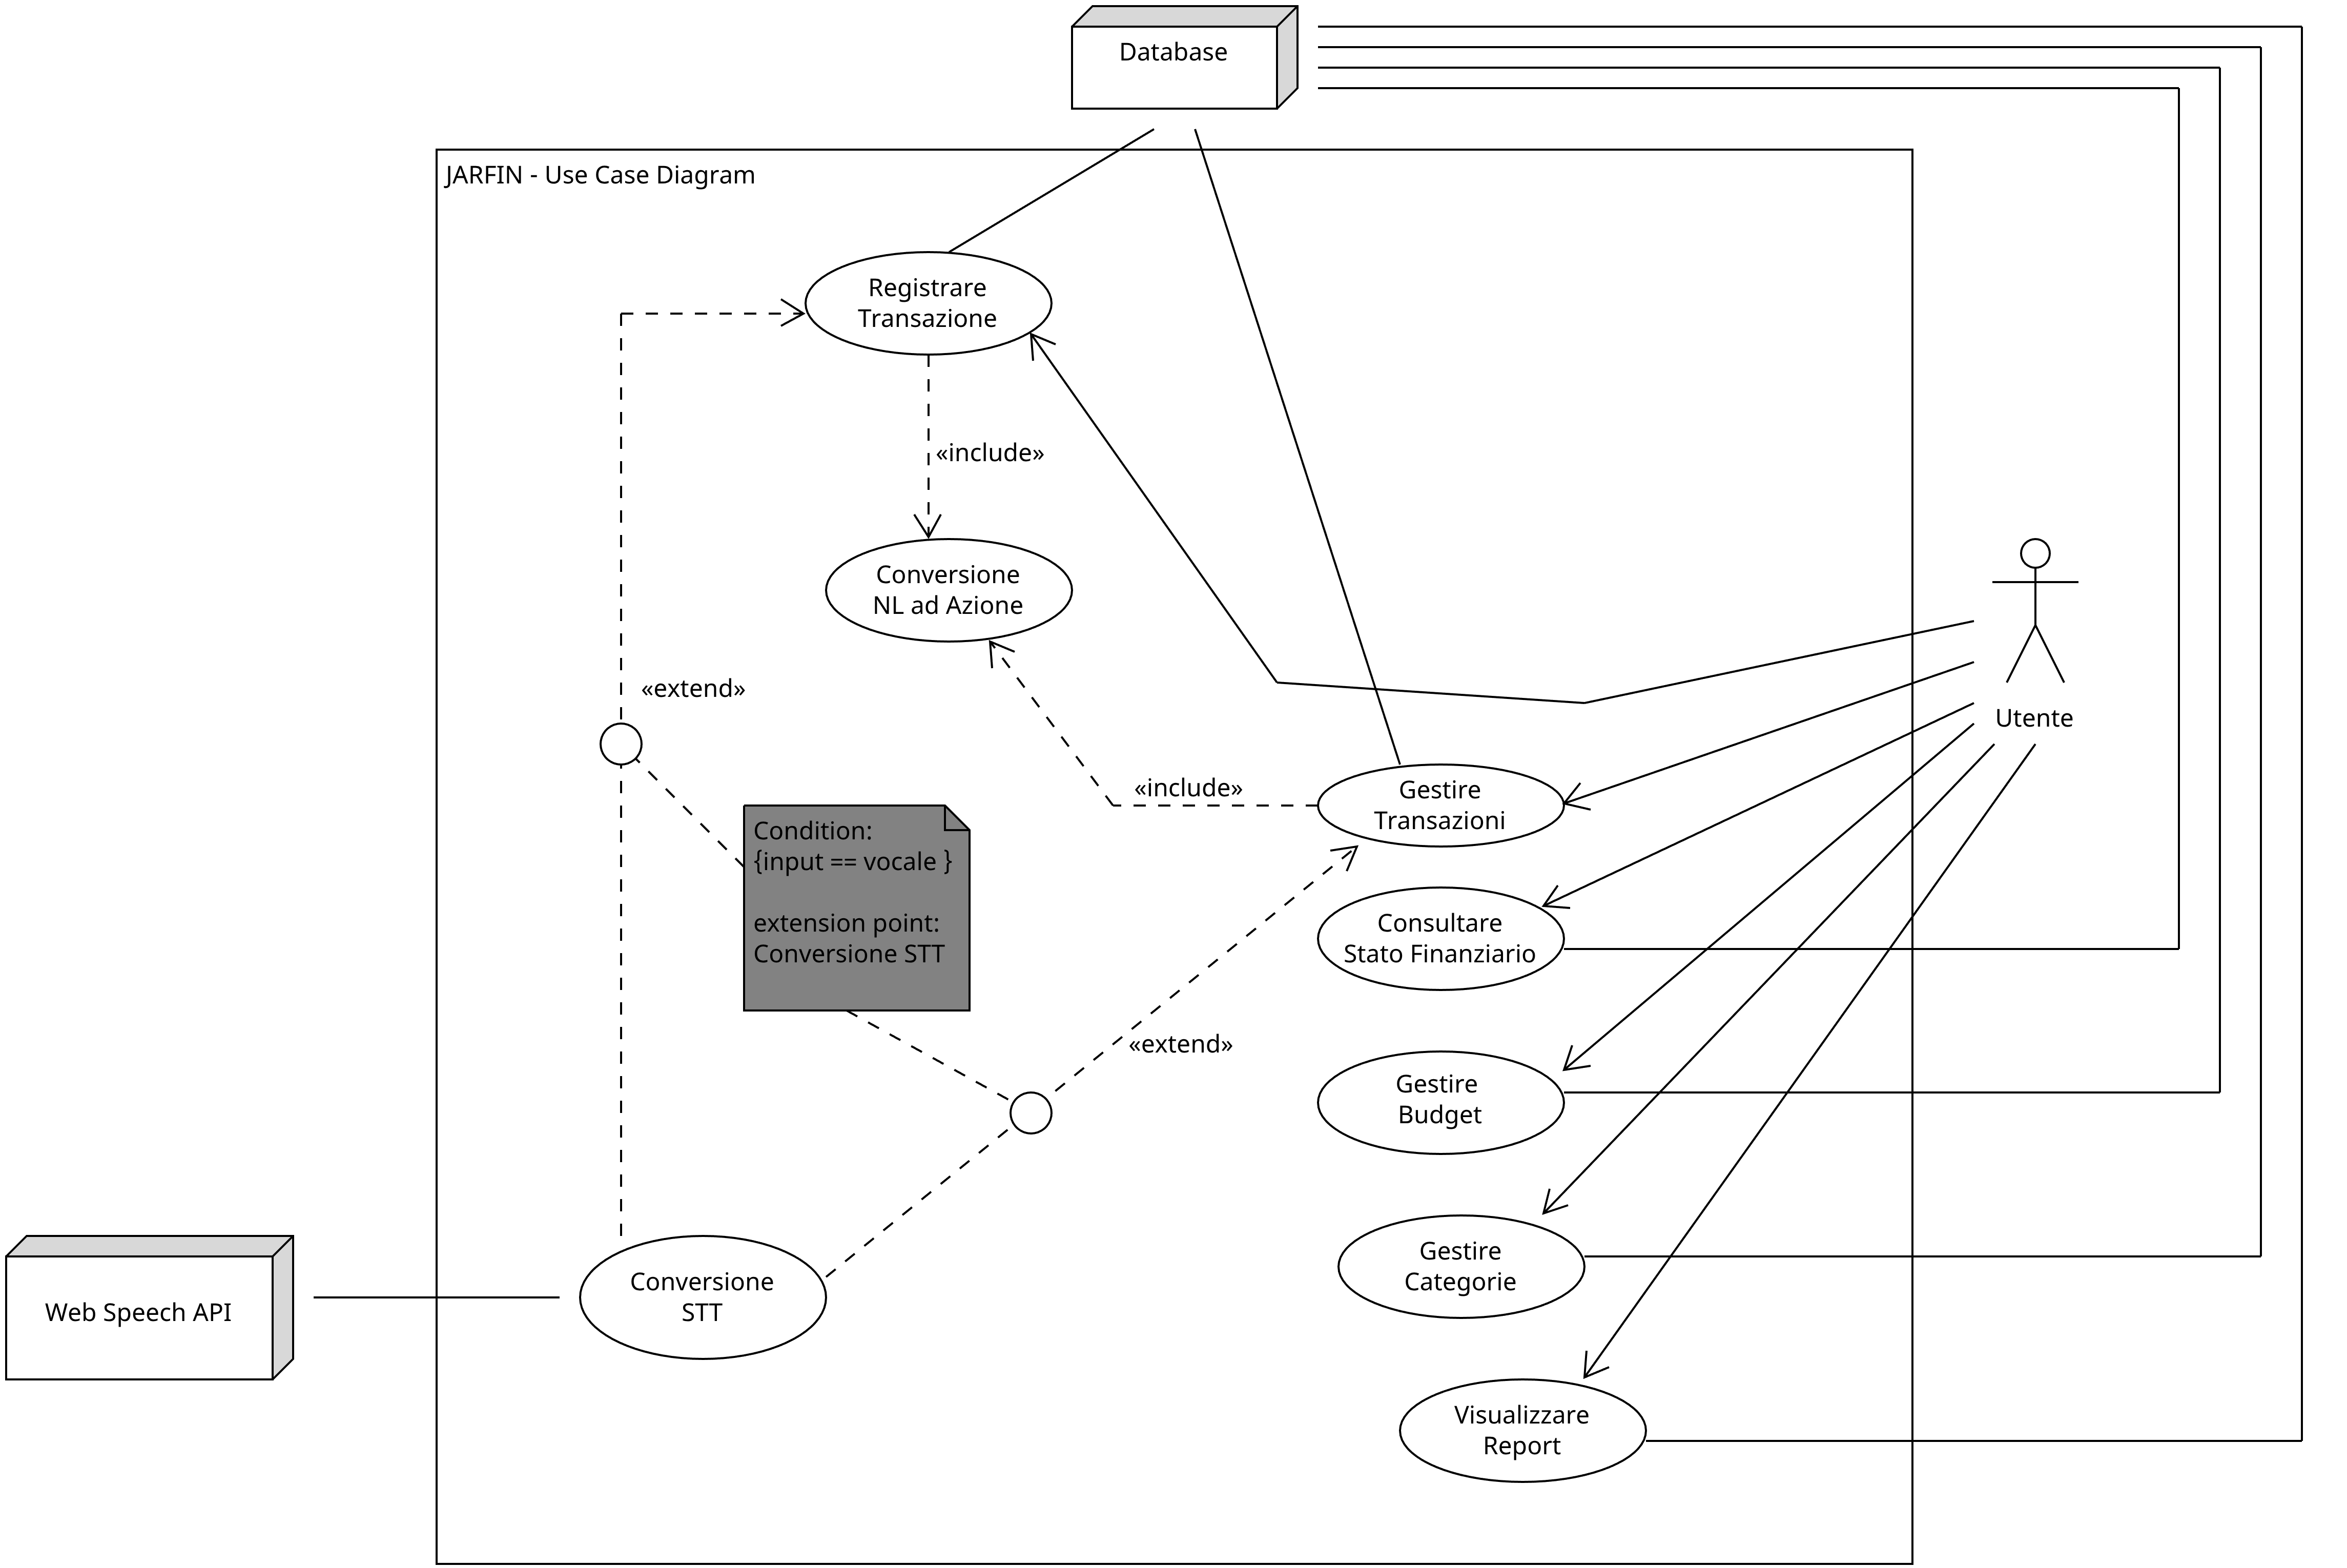
\includegraphics[width=1\textwidth]{../Iterazione_0/images/use_case_diagram.png}
    \caption{Diagramma dei casi d'uso (Vista degli Scenari).}
    \label{fig:use_case}
\end{figure}

\subsection{Attori}
Il diagramma identifica due tipologie di attori:
\begin{itemize}
    \item \textbf{Utente}: attore primario che interagisce con l'interfaccia web per la gestione delle proprie finanze.
    \item \textbf{Sistemi esterni}: attori secondari necessari al funzionamento del backend:
          \begin{itemize}
              \item \textbf{Cloud Speech-to-Text}: servizio invocato per la trascrizione dei comandi vocali;
              \item \textbf{Database}: sistema responsabile della persistenza fisica di tutte le entità (utenti, transazioni, categorie).
          \end{itemize}
\end{itemize}

\subsection{Descrizione dei Casi d'Uso}

Le funzionalità sono state raggruppate in tre macro-aree logiche per facilitarne la lettura e l'implementazione.



\subsubsection{Gestione Transazioni}
Rappresenta il nucleo operativo dell'applicazione (\textit{Core Domain}).
\begin{itemize}
    \item \textbf{Registrare Transazione}: permette l'inserimento di una nuova spesa o entrata.
          \begin{itemize}
              \item \textit{Inclusione («include»)}: include obbligatoriamente il caso d'uso \textbf{"Conversione NL ad Azione"}, poiché ogni input (testuale o vocale) deve essere processato dal parser NLU per estrarre i dati strutturati.
              \item \textit{Estensione («extend»)}: è esteso da \textbf{"Conversione STT"} se la condizione \texttt{input == vocale} è soddisfatta.
          \end{itemize}
    \item \textbf{Gestire Transazioni}: permette la modifica o l'eliminazione di movimenti esistenti.
          \begin{itemize}
              \item Anche questo caso d'uso include la logica di parsing NLU ed è esteso dalla conversione vocale, permettendo all'utente di modificare i dati tramite comandi vocali.
          \end{itemize}
\end{itemize}

\subsubsection{Analisi e Configurazione}
Riguarda le funzionalità di monitoraggio e organizzazione dei dati.
\begin{itemize}
    \item \textbf{Consultare Stato Finanziario}: visualizzazione immediata del saldo attuale.
    \item \textbf{Gestire Budget}: definizione dei limiti di spesa mensili.
    \item \textbf{Gestire Categorie}: permette all'utente di creare, modificare o eliminare le categorie di spesa personalizzate (es. "Svago", "Casa").
    \item \textbf{Visualizzare Report}: generazione di un report mensili per l'utente.
\end{itemize}

\section{Vista logica – Class Diagram}

La vista logica (Figura \ref{fig:classdiagram}) illustra la struttura statica del sistema, evidenziando la suddivisione in microservizi e le relazioni tra le classi. Il diagramma riflette l'architettura modulare adottata, dove ogni componente ha responsabilità ben definite.

\begin{figure}[H]
    \centering
    \includegraphics[width=0.83\textwidth]{../Iterazione_0/images/class_diagram.png}
    \caption{Diagramma di classi (Vista Logica).}
    \label{fig:classdiagram}
\end{figure}

\newpage
\subsection{Shared Kernel e Modello di Dominio}
L'entità core del sistema è definita all'interno del servizio di Accounting:
\begin{itemize}
    \item \textbf{\texttt{Transaction}}: Rappresenta l'entità fondamentale mappata sul database. Include i campi \texttt{id} (Long), \texttt{amount} (BigDecimal), \texttt{date} (LocalDate), \texttt{description} (String), \texttt{category} (String) e \texttt{type} (Enum INCOME/EXPENSE).
\end{itemize}

\subsection{Web UI e NLU Service}
Questo modulo gestisce l'interfaccia utente e l'interpretazione dei comandi vocali:
\begin{itemize}
    \item \textbf{\texttt{CommandController} e \texttt{HomeController}}: Ricevono le richieste dal frontend. Il \texttt{CommandController} elabora i payload vocali invocando localmente il servizio NLU e successivamente usa il \texttt{RestTemplate} per instradare le richieste al Gateway.
    \item \textbf{\texttt{NaturalLanguageService}}: Il componente core che esegue il parsing del testo utilizzando pattern predefiniti e mappe di categorie per estrarre i dati transazionali.
    \item \textbf{\texttt{ParsedTransaction}}: Data Transfer Object (DTO) che racchiude l'intento estratto, includendo il \texttt{CommandType} (CREATE, DELETE, UPDATE) e i dati della transazione.
\end{itemize}

\subsection{Analytics Service}
Localizzato nel package dedicato, si occupa della generazione della reportistica finanziaria:
\begin{itemize}
    \item \textbf{\texttt{AnalyticsController}}: Espone l'endpoint \texttt{getReport()} che restituisce un oggetto di tipo \texttt{FinancialReportDTO}.
    \item \textbf{\texttt{AnalyticsService}}: Contiene la logica per richiedere le transazioni all'Accounting Service (via \texttt{RestTemplate}) e aggregare i dati tramite il metodo \texttt{generateReport()}.
    \item \textbf{\texttt{FinancialReportDTO}}: Struttura dati ottimizzata per il frontend che include \texttt{totalBalance}, \texttt{totalIncomes}, \texttt{totalExpenses} e \texttt{breakdownByCategory}.
\end{itemize}

\subsection{Accounting Service}
Modulo preposto alla gestione della persistenza e della logica transazionale:
\begin{itemize}
    \item \textbf{\texttt{TransactionController}}: Punto di ingresso per le operazioni CRUD (\texttt{create}, \texttt{findAll}, \texttt{getById}, \texttt{update}, \texttt{delete}).
    \item \textbf{\texttt{TransactionService}}: Implementa i metodi operativi come \texttt{saveTransaction()}, \texttt{updateTransaction()} e \texttt{deleteTransaction()}.
    \item \textbf{\texttt{TransactionRepository}}: Interfaccia Spring Data JPA per l'accesso diretto ai dati su PostgreSQL.
\end{itemize}

\subsection{Orchestrazione e API Gateway}
L'architettura utilizza un \textbf{\texttt{JarfinApiGatewayApplication}}:
\begin{itemize}
    \item \textbf{Routing}: Funge da unico punto di accesso per le API di backend, instradando le richieste provenienti dalla Web UI verso i controller di \texttt{Accounting} e \texttt{Analytics}.
\end{itemize}

\newpage
\section{Vista di sviluppo – Component Diagram}

Il Diagramma dei Componenti (Figura \ref{fig:components}) illustra l'organizzazione del sistema JarFin in moduli software distinti e le dipendenze che intercorrono tra di essi. Questa vista evidenzia una struttura a tre livelli (\textit{Layered Architecture}):

\begin{figure}[H]
    \centering
    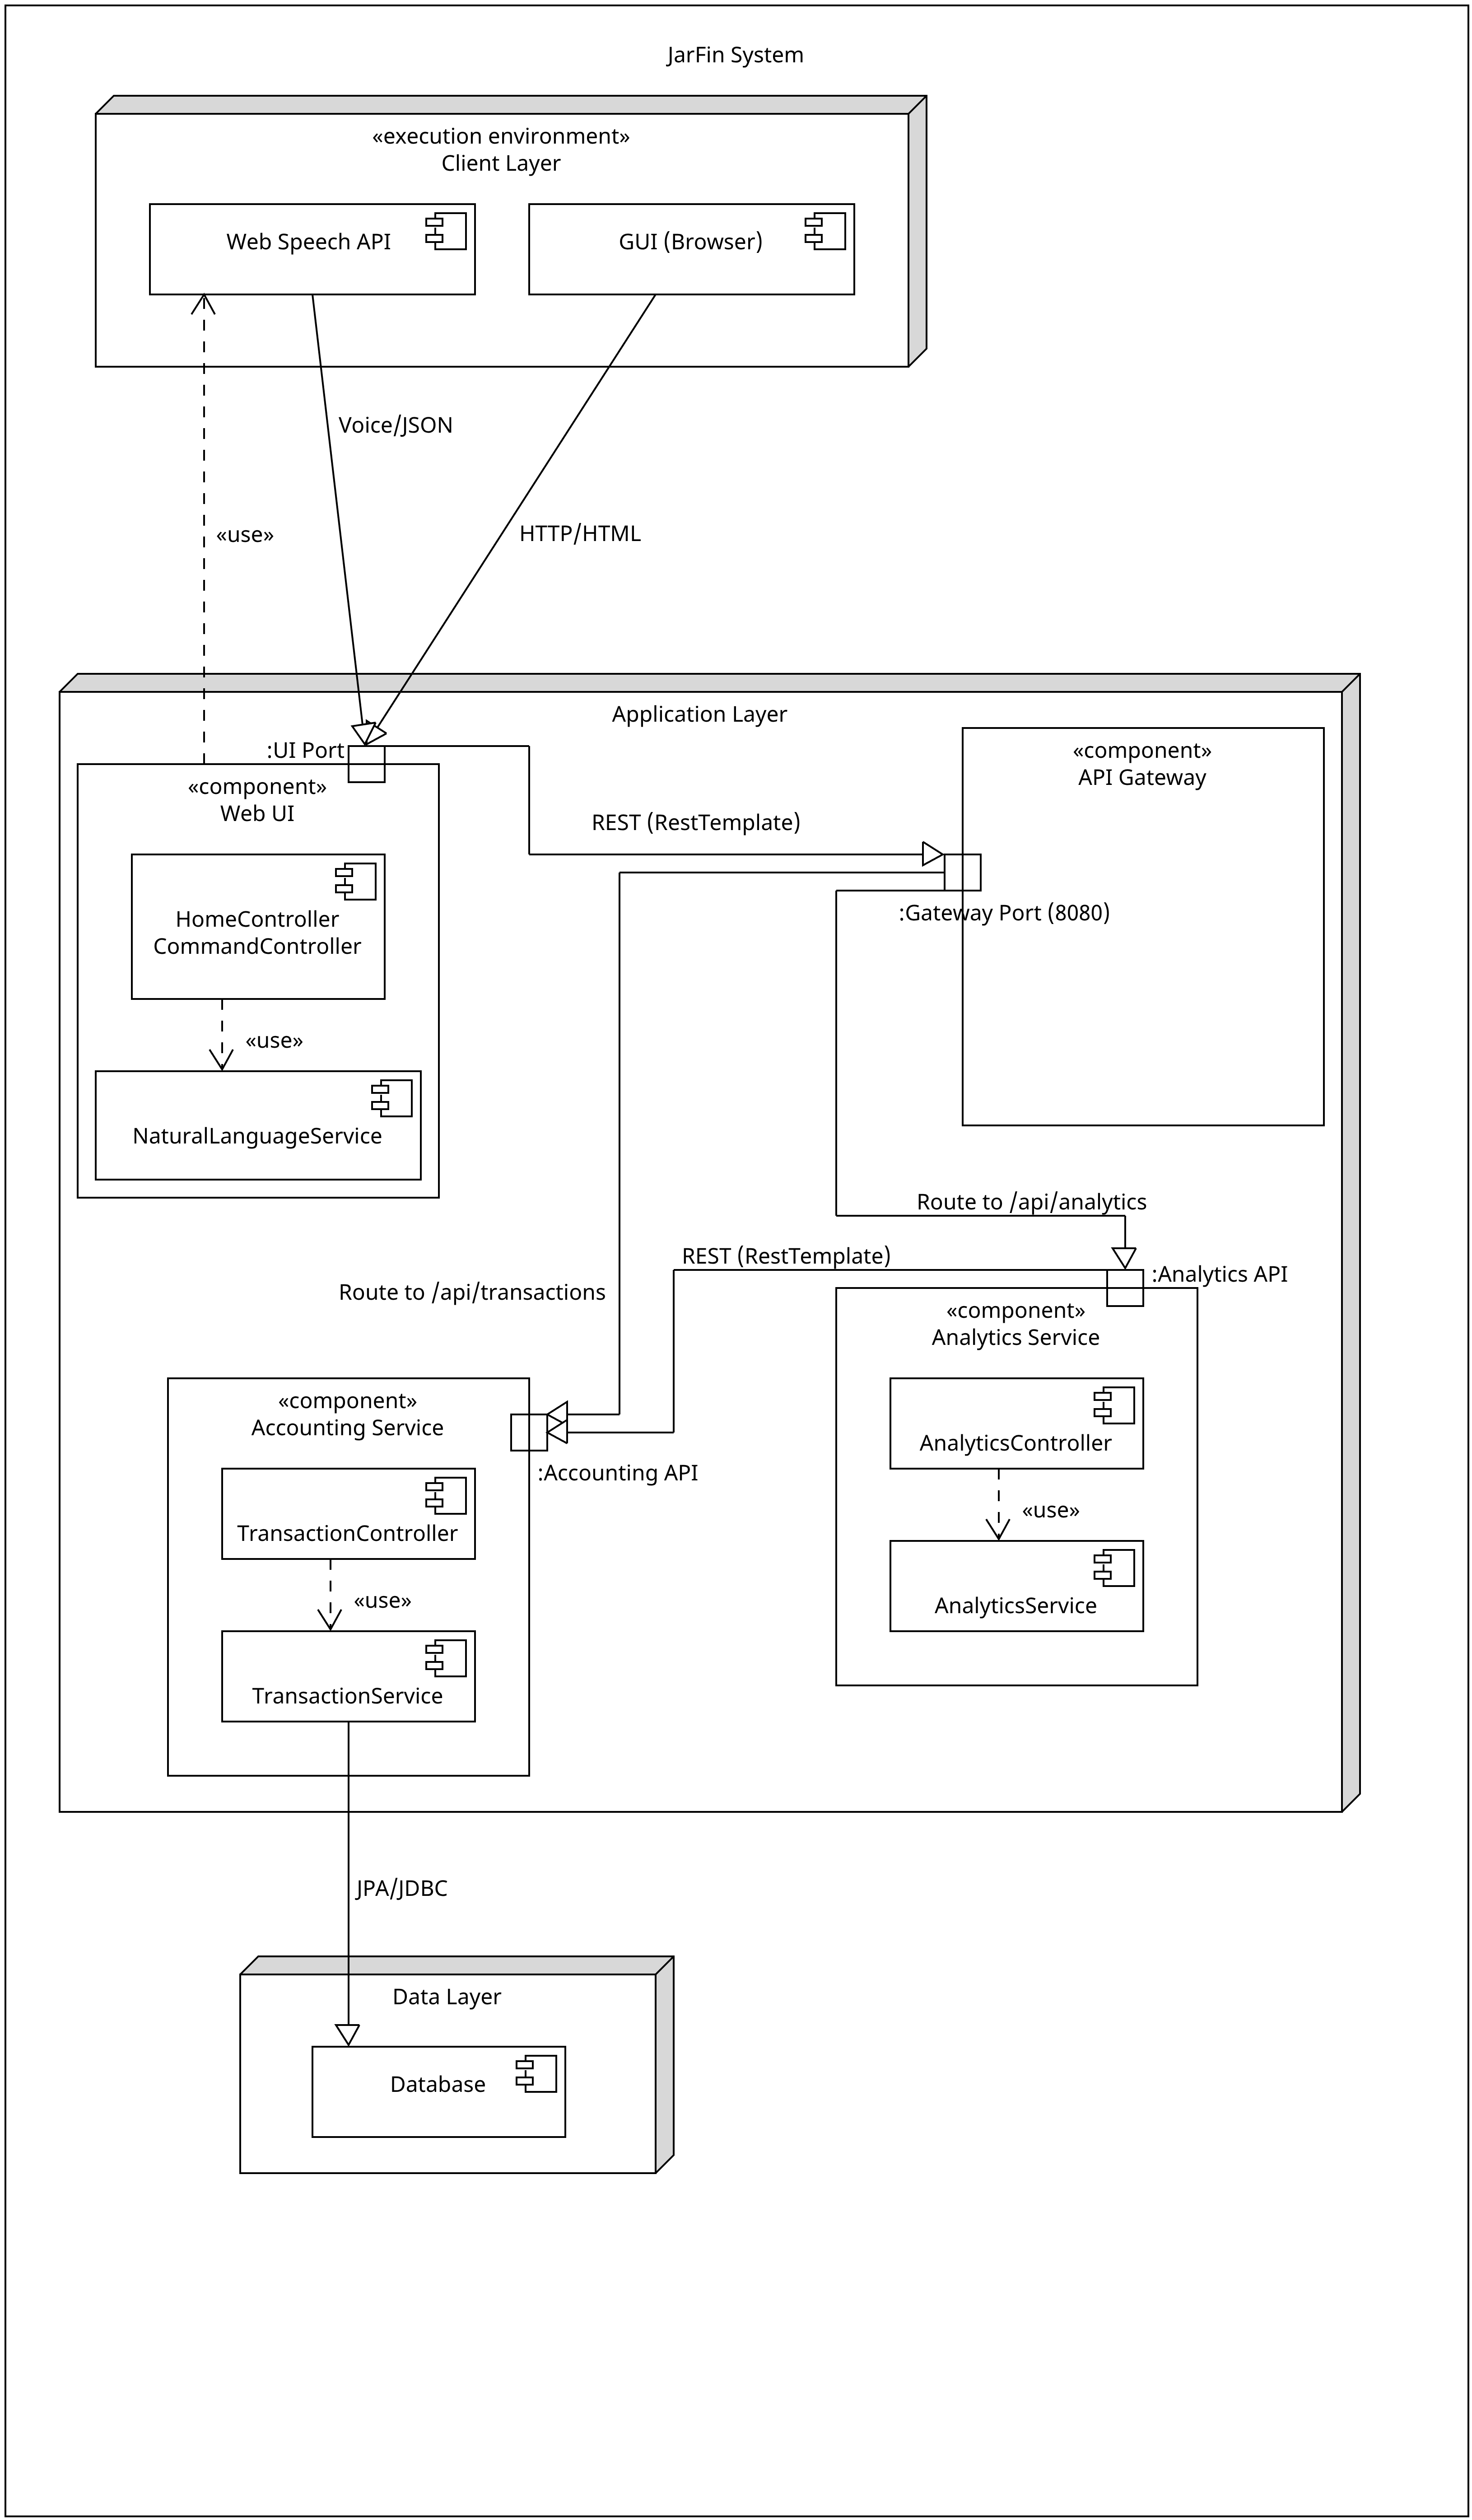
\includegraphics[width=0.65\textwidth]{../Iterazione_0/images/component_diagram.png}
    \caption{Diagramma dei componenti: architettura a livelli e interfacce esposte.}
    \label{fig:components}
\end{figure}

\subsection{Client Layer}
Il livello superiore rappresenta il frontend e i servizi di interazione immediata con l'utente:
\begin{itemize}
    \item \textbf{GUI}: Componente che gestisce la logica di visualizzazione, implementando l'interfaccia \texttt{UserInterface} con i metodi \texttt{inputCommand()} e \texttt{displayReport()}.
    \item \textbf{Web Speech API (Browser)}: Componente che fornisce le capacità di riconoscimento vocale integrate nel browser.
    \item \textbf{Porte}: La comunicazione verso i livelli sottostanti è veicolata tramite la \texttt{GUIPORT [1]}.
\end{itemize}

\subsection{Application Layer}
Il nucleo del sistema incapsula la logica di business ed è suddiviso in quattro moduli principali (microservizi):
\begin{itemize}
    \item \textbf{Web UI}: Contiene i controller web e incapsula il \texttt{NaturalLanguageService}. Funge da Backend For Frontend (BFF).
    \item \textbf{API Gateway}: Il punto di ingresso centralizzato che instrada il traffico verso i microservizi di dominio.
    \item \textbf{Accounting Service}: Gestisce i flussi finanziari e la logica CRUD esponendo le proprie API REST.
    \item \textbf{Analytics Service}: Aggrega i dati interrogando l'Accounting Service per calcolare le statistiche.
\end{itemize}

\subsection{Data Layer}
Il livello di persistenza è isolato dal resto dell'applicazione per garantire l'indipendenza dallo storage:
\begin{itemize}
    \item \textbf{Database}: Componente responsabile dell'archiviazione dei dati.
    \item \textbf{DBInterface}: L'interfaccia di accesso ai dati che astrae le operazioni CRUD fondamentali: \texttt{save()}, \texttt{findAll()}, \texttt{findById()} e \texttt{deleteById()}.
    \item \textbf{Porte}: Riceve le richieste dal livello applicativo sulla porta \texttt{DBPORT [1]} attraverso una connessione verso la \texttt{DatabasePort}.
\end{itemize}

\subsection{Dipendenze e Relazioni}
\begin{itemize}
    \item \textbf{Relazione di Uso}: Il componente \texttt{Web UI} presenta una dipendenza \texttt{«use»} verso la \texttt{Web Speech API} del Client Layer per le funzionalità STT.
    \item \textbf{Integrazione e Routing}: La \texttt{Web UI} comunica con l'\texttt{API Gateway}, che a sua volta instrada verso \texttt{Accounting} e \texttt{Analytics}. L'\texttt{Analytics Service} interroga l'\texttt{Accounting Service} per ottenere i dati necessari all'aggregazione.
\end{itemize}

\section{Vista di processo – Sequence Diagram}

La vista di processo descrive la dinamica temporale delle interazioni tra gli attori e i componenti del sistema JarFin durante l'esecuzione di un comando. Il diagramma (Figura \ref{fig:sequence}) illustra il flusso completo, dalla ricezione dell'input alla persistenza dei dati e alla generazione del feedback.

\begin{figure}[H]
    \centering
    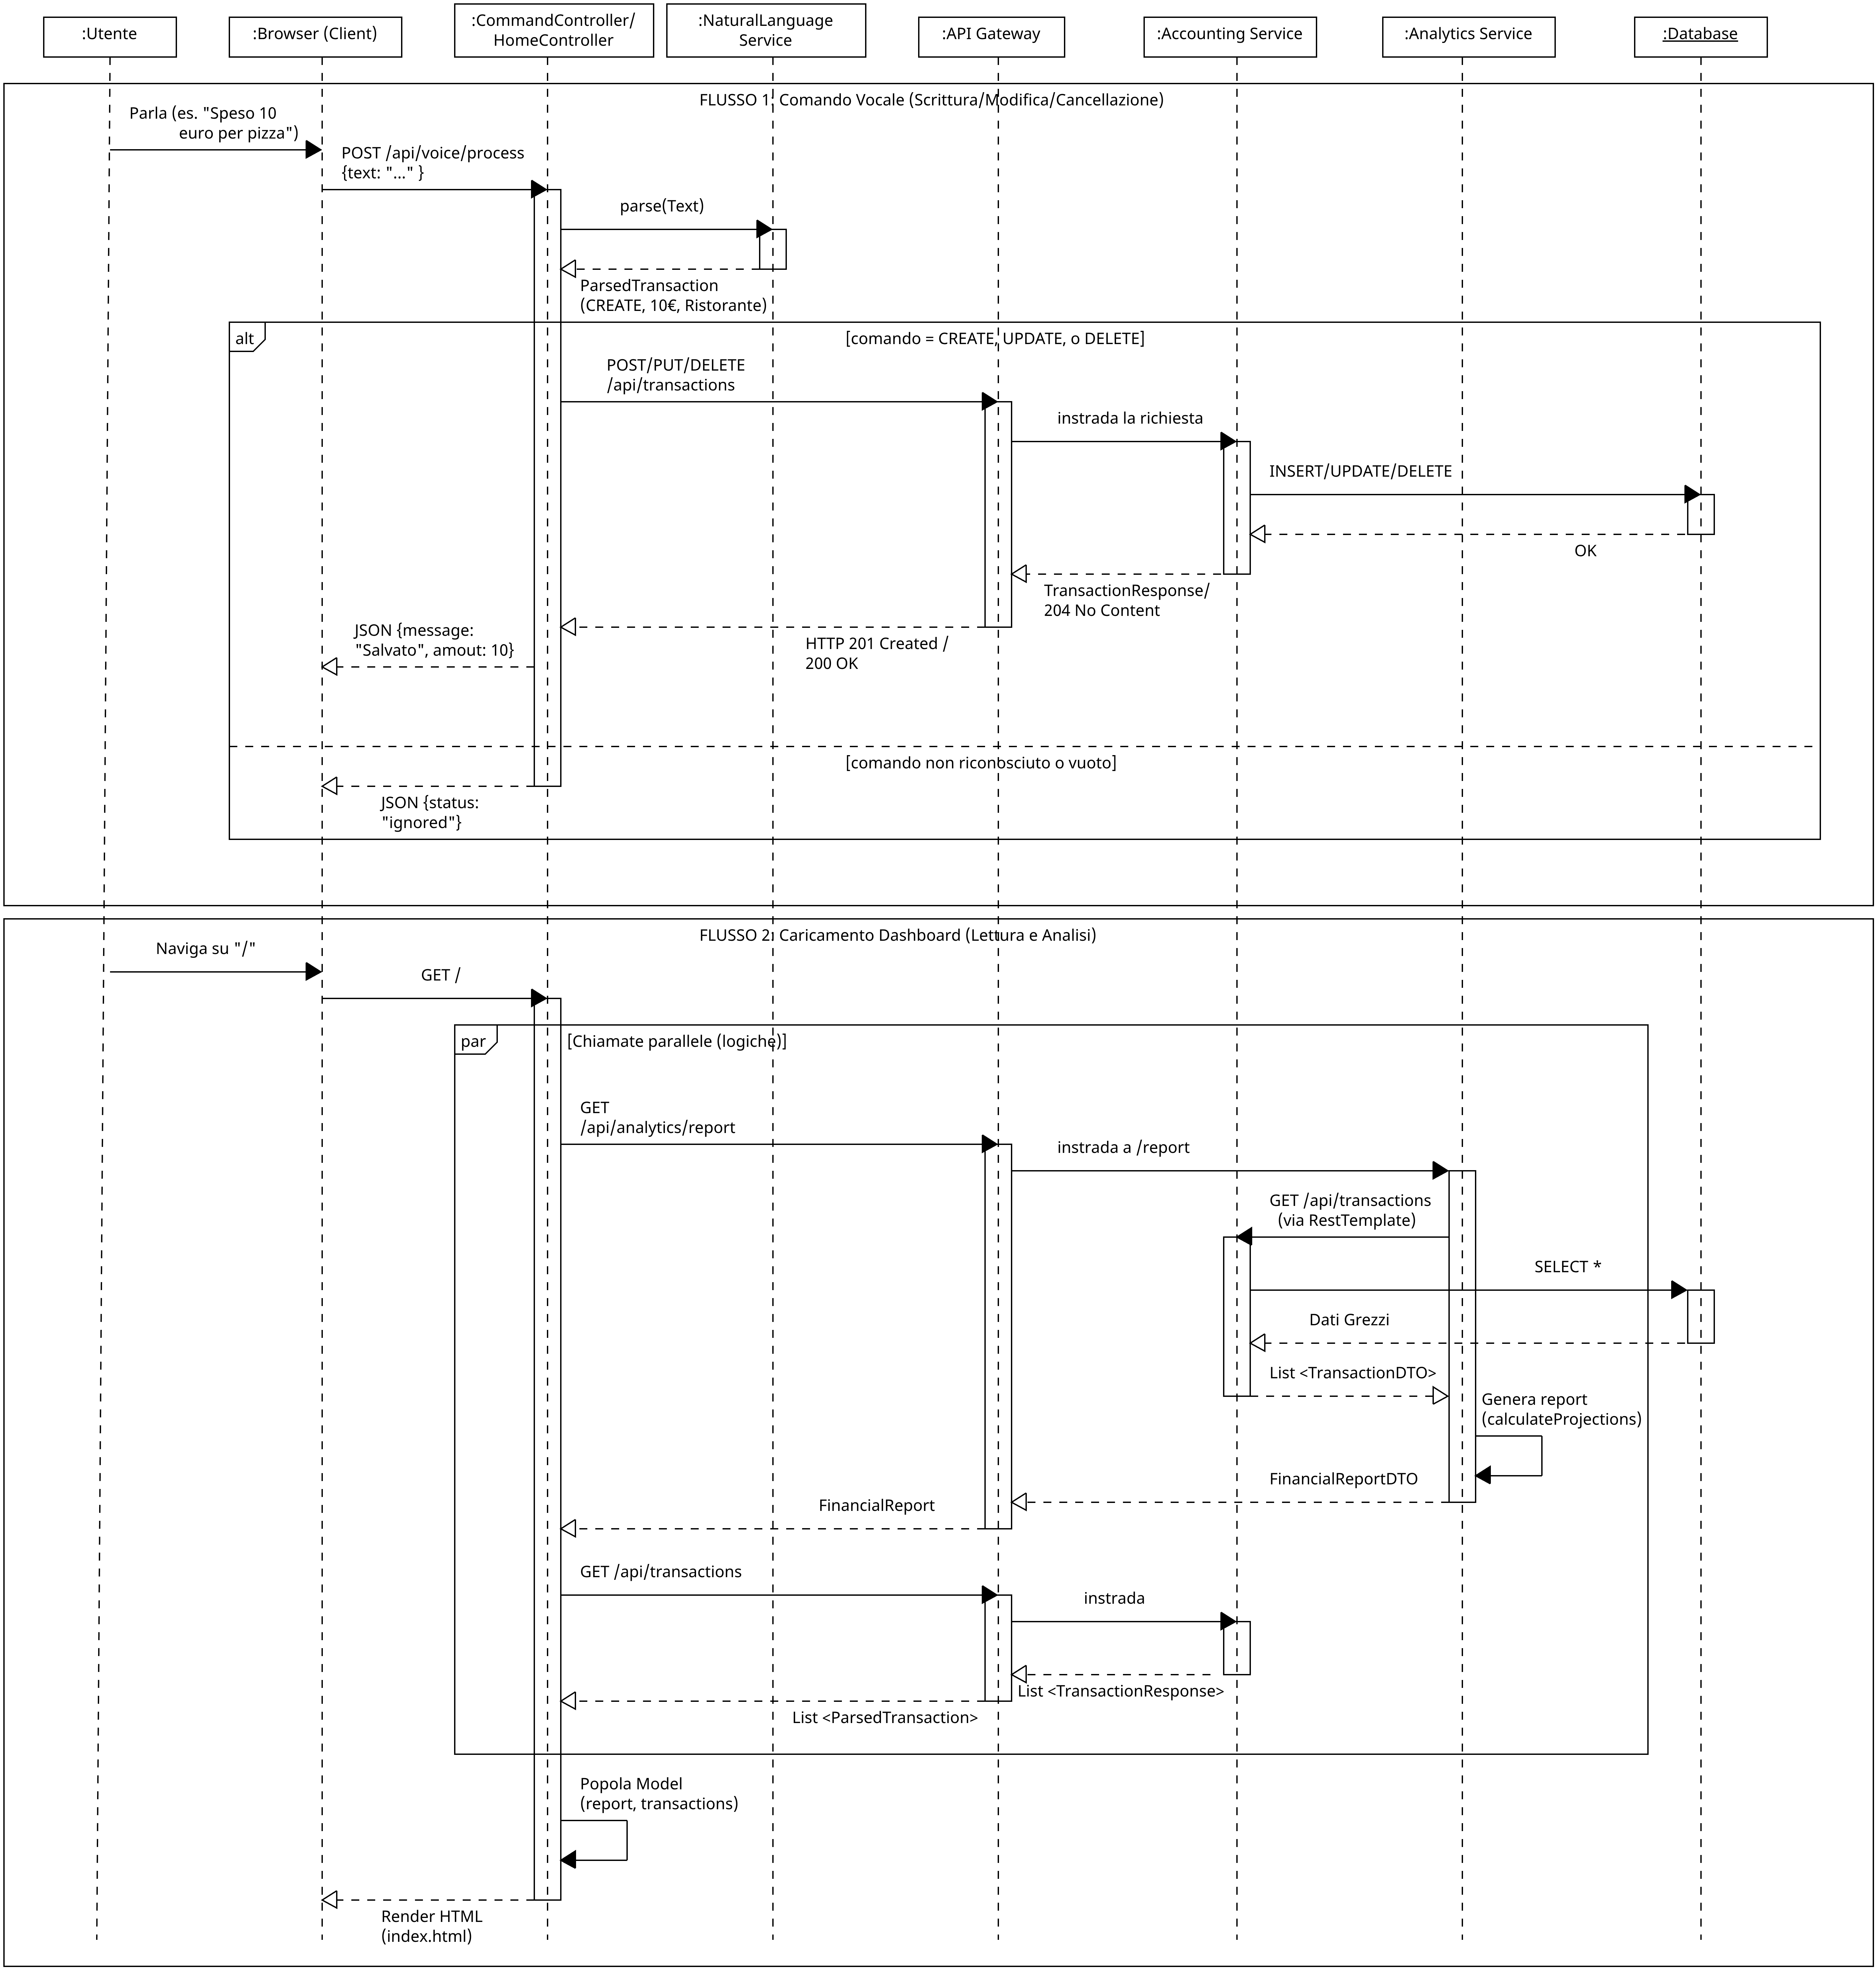
\includegraphics[width=0.79\textwidth]{../Iterazione_0/images/sequence_diagram.png}
    \caption{Diagramma di sequenza: autenticazione, gestione comandi e routing.}
    \label{fig:sequence}
\end{figure}

\subsection{Fase 1: Input e Comando Vocale}
Il flusso per l'inserimento o la modifica tramite voce ha inizio con l'interazione dell'utente:
\begin{enumerate}
    \item \textbf{Invio Comando}: L'utente parla, il browser converte l'audio in testo e lo invia alla \texttt{Web UI} tramite \texttt{POST /api/voice/process}.
    \item \textbf{Analisi Semantica}: Il Controller invoca localmente il \texttt{NaturalLanguageService} per estrarre l'intento e i dati.
    \item \textbf{Inoltro al Gateway}: La \texttt{Web UI} inoltra la richiesta strutturata all'\texttt{API Gateway}, che la instrada all'\textbf{Accounting Service}.
    \item \textbf{Persistenza}: L'Accounting Service esegue l'operazione (INSERT/UPDATE/DELETE) sul Database, che restituisce conferma. L'esito risale fino alla Web UI.
\end{enumerate}

\subsection{Fase 2: Caricamento Dashboard (Lettura e Analisi)}
Quando l'utente visita la pagina principale per consultare i report:
\begin{itemize}
    \item La \texttt{Web UI} richiede il report all'\texttt{API Gateway}, che instrada la chiamata all'\textbf{Analytics Service}.
    \item L'\textbf{Analytics Service} effettua una chiamata REST all'\textbf{Accounting Service} per ottenere la lista delle transazioni correnti.
    \item L'Accounting Service interroga il \texttt{Database} (\texttt{SELECT}), ottiene i dati grezzi e li restituisce.
    \item Ricevuti i dati, l'Analytics calcola i totali e le proiezioni, restituendo il \texttt{FinancialReport} alla \texttt{Web UI} per il rendering HTML.
\end{itemize}

\subsection{Fase 3: Feedback Finale}
Una volta completata l'elaborazione nei microservizi, il ciclo si conclude con la notifica all'utente:
\begin{enumerate}
    \item L'\texttt{Api Gateway} invia la \texttt{Risposta Utente} alla \texttt{Web UI}.
    \item L'applicazione mostra il \texttt{Feedback} finale (sotto forma di testo e interfacce aggiornate) all'utente.
\end{enumerate}

\section{Vista fisica – Deployment Diagram}

Il Diagramma di Deployment (Figura \ref{fig:deployment}) illustra la distribuzione fisica del sistema JarFin, mappando gli artefatti software sui nodi hardware e descrivendo i protocolli di comunicazione utilizzati.

\begin{figure}[H]
    \centering
    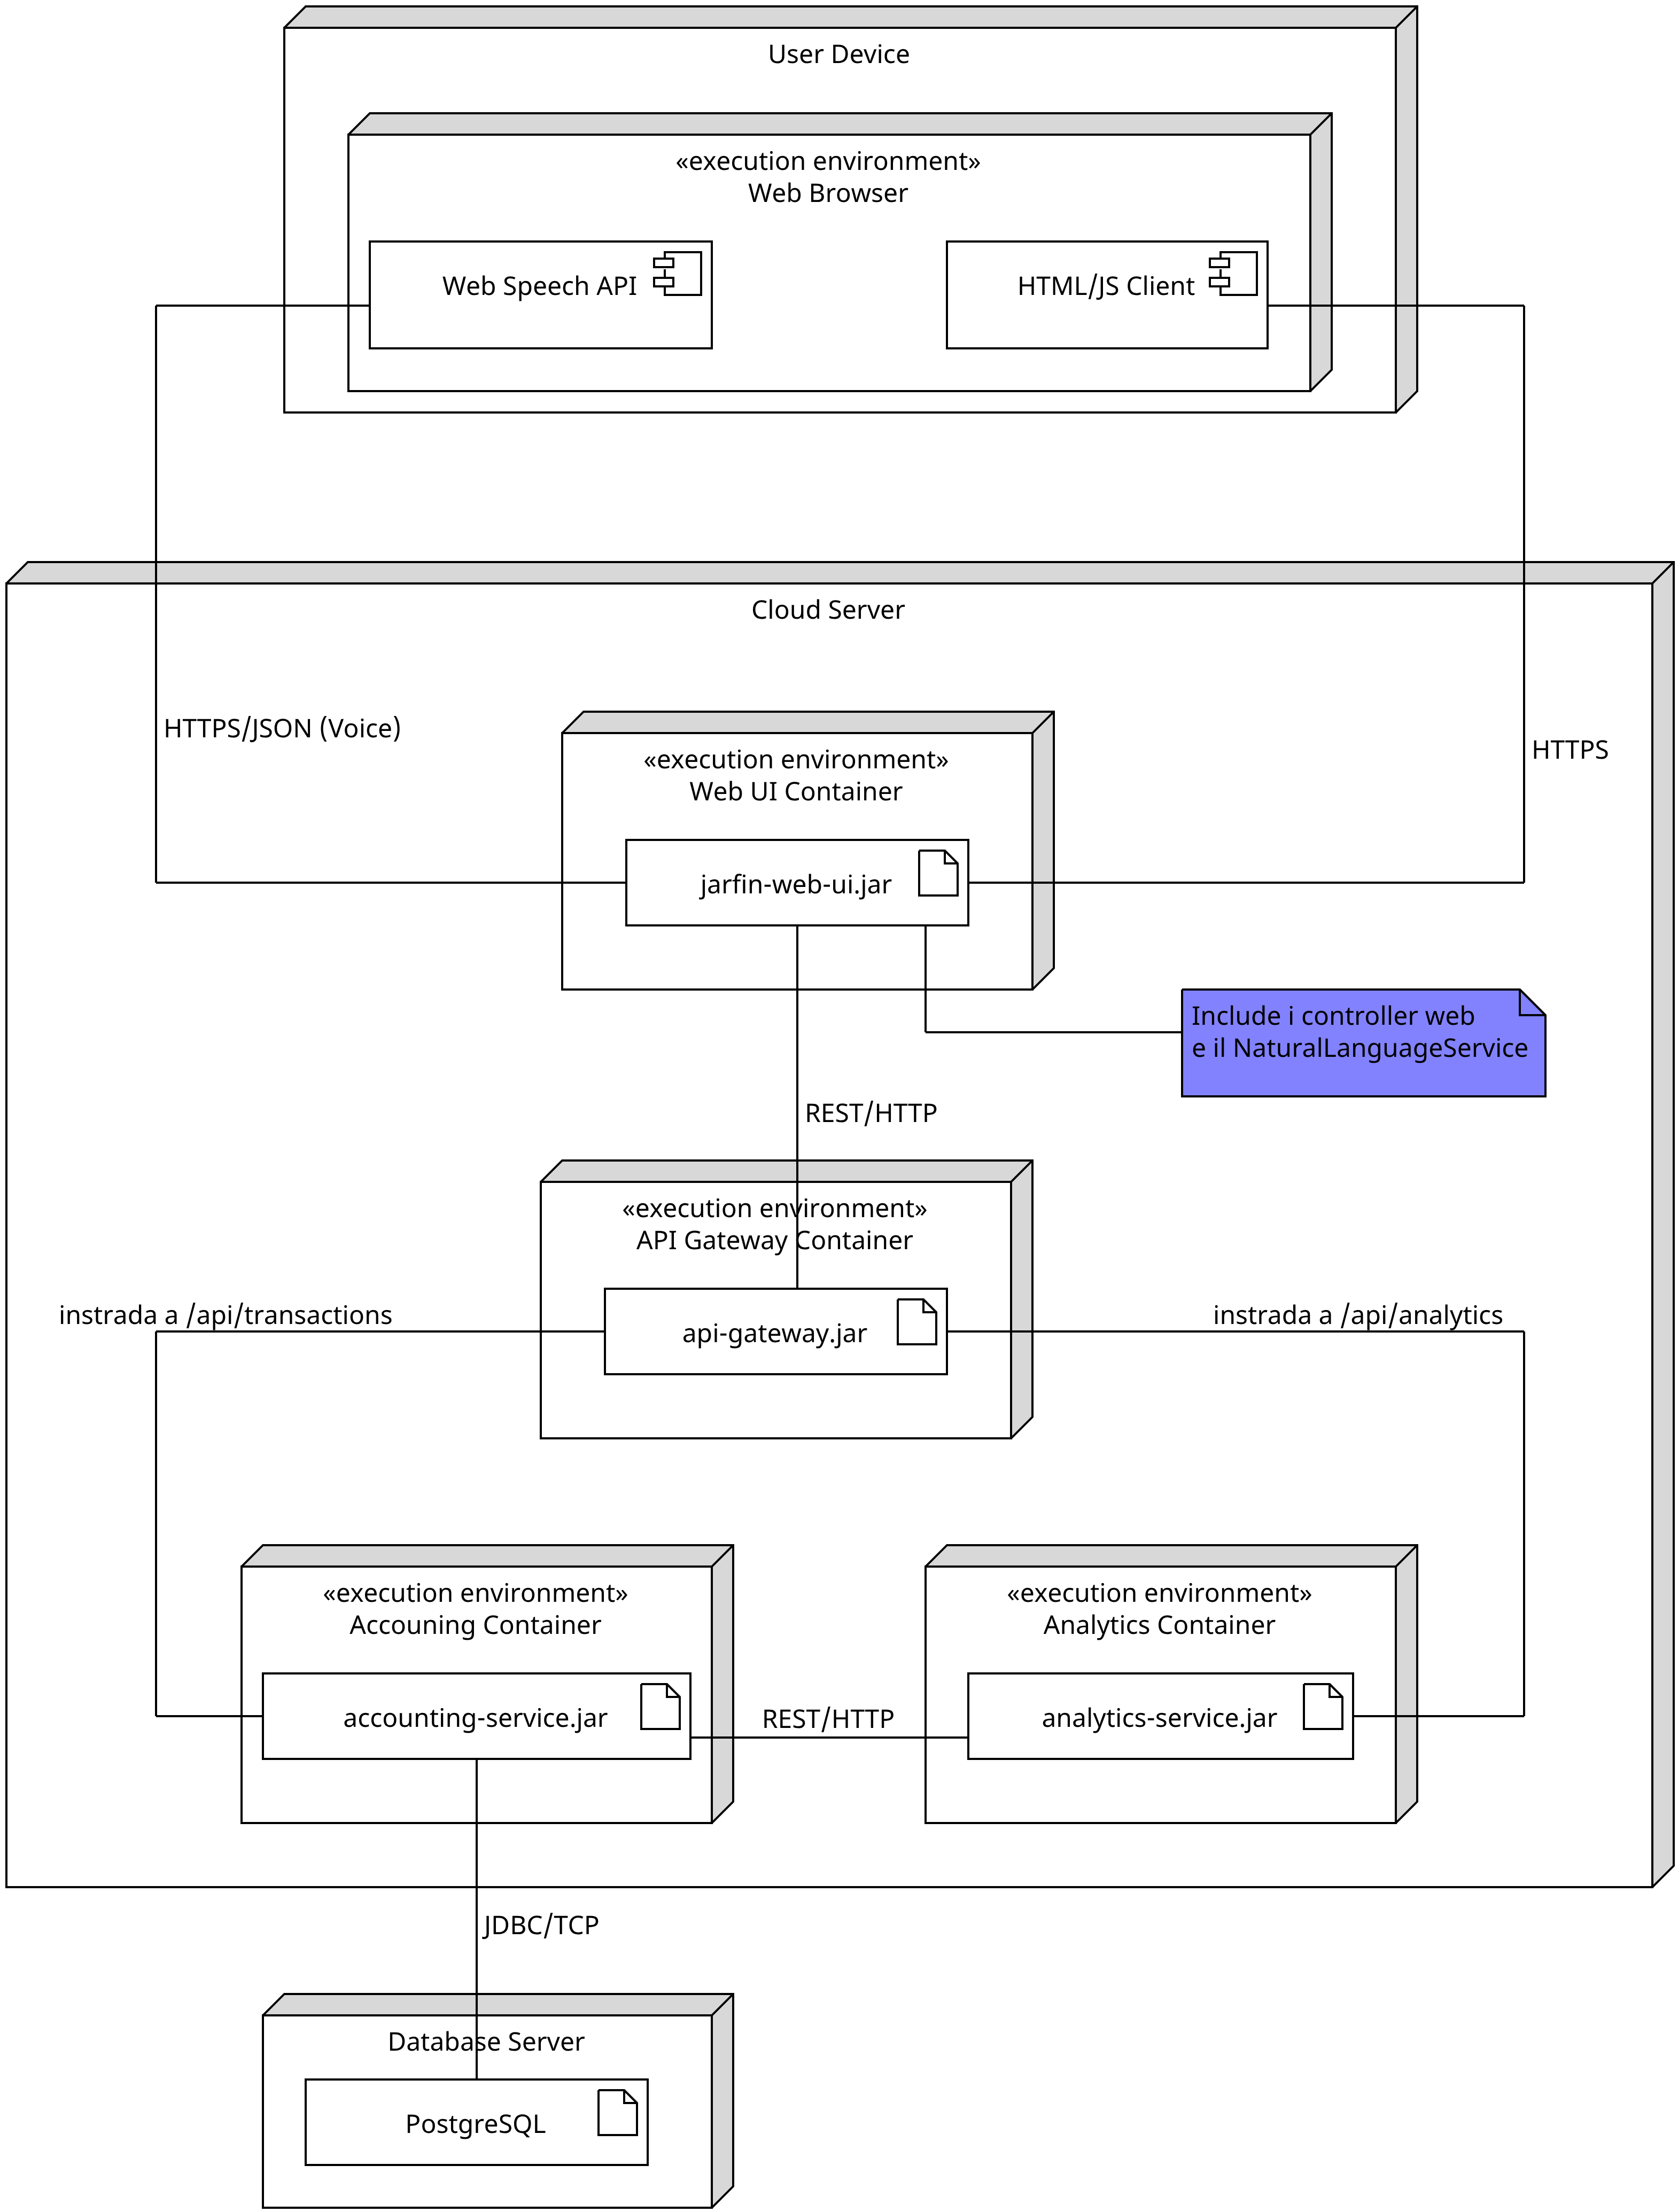
\includegraphics[width=0.7\textwidth]{../Iterazione_0/images/deployment_diagram.png}
    \caption{Diagramma di deployment: nodi fisici, container e protocolli di rete.}
    \label{fig:deployment}
\end{figure}

\subsection{Architettura dei Nodi e Ambienti}
Il sistema è distribuito su infrastrutture distinte che separano il frontend, la logica applicativa e la persistenza:

\begin{itemize}
    \item \textbf{User Device}: Rappresenta il dispositivo terminale dell'utente. Ospita l'ambiente di esecuzione \textbf{Web Browser} con le interfacce client e sfrutta la \textbf{Web Speech API} per la conversione locale dell'audio in testo (STT).

    \item \textbf{Cloud Server}: Il nodo centrale che ospita il backend Java Spring Boot. È suddiviso in ambienti di esecuzione containerizzati per garantire l'isolamento:
          \begin{itemize}
              \item \textbf{Web UI Container}: Esegue l'artefatto \texttt{jarfin-web-ui.jar} (che include la logica NLU e serve le pagine web).
              \item \textbf{API Gateway Container}: Esegue l'artefatto \texttt{api-gateway.jar}.
              \item \textbf{Accounting Container}: Esegue l'artefatto \texttt{accounting-service.jar}.
              \item \textbf{Analytics Container}: Esegue l'artefatto \texttt{analytics-service.jar}.
          \end{itemize}

    \item \textbf{Database Server}: Un nodo dedicato che ospita il DBMS \textbf{PostgreSQL}, garantendo che la persistenza dei dati sia fisicamente separata dalla logica di business per ottimizzare sicurezza e performance.
\end{itemize}

\subsection{Protocolli di Comunicazione}
Le interconnessioni tra i vari nodi utilizzano protocolli standard per lo scambio di dati:

\begin{itemize}
    \item \textbf{User Device $\xrightarrow{HTTPS/JSON}$ Cloud Server}: La comunicazione tra il browser dell'utente e il server applicativo avviene tramite il protocollo \textbf{HTTPS}. I dati vengono scambiati in formato \textbf{JSON}, permettendo al client di inviare comandi e ricevere report o conferme.

    \item \textbf{Cloud Server $\xrightarrow{JDBC}$ Database Server}: L'accesso ai dati da parte dei microservizi (in particolare il servizio Accounting) avviene tramite una connessione \textbf{JDBC} verso l'istanza di PostgreSQL.

    \item \textbf{Integrazione Locale}: A differenza di implementazioni puramente cloud, il diagramma evidenzia che la componente di trascrizione vocale (\textbf{Web Speech API}) risiede nello \textit{User Device}, riducendo la necessità di inviare flussi audio grezzi verso nodi esterni per il solo STT.
\end{itemize}

\section{Conclusioni dell'Iterazione 0}

L'attività di analisi e progettazione ha prodotto un'architettura solida, modulare e documentata. L'adozione del modello 4+1 ha permesso di affrontare la complessità del sistema distribuito, definendo chiaramente le responsabilità di ogni componente prima dell'inizio della fase di codifica (Iterazione 1).